% !TEX root =  sc19-main.tex


\section[Introduction]{Introduction}

% Study on old supercomputers (Athena, Jaguar, Jaguar Petaflop,
% Kraken)
%   https://ieeexplore.ieee.org/stamp/stamp.jsp?tp=&arnumber=7448082
%   Emergency Actions over one year: 35 for Athena, 58 for Jaguar, 130
%   for Jaguar PetaFlops, 53 for Kraken
%  The paper mostly discusses emergency maintenance vs preventive
%  maintenance. Preventive maintenance had a positive effect on the
%  reliability of the hardware only when the actual root cause of
%  failure could be identified (Jaguar); other preventive maintenance
%  had sometimes an adverse effect on the reliability
%  (Athena). Emergency maintenance has only for effect to restore the
%  behavior and has no impact on the MTBF (hypothesis of memoryless
%  seems to be validated in that case).

% Mistral supercomputer job history analysis
% https://arxiv.org/pdf/1801.07624.pdf
%   Two types of failures: node-fail = crash of a computing node
%   detected by timeout of a watchdog on the OS of the node,
%   failed-job = any reason the job returned a negative code,
%   including failures of the filesystem or other components (not
%   node). 
%    0.028% of jobs fail because of a computing node timeout
%    390 node_fail jobs, strong correlation between duration and
%    number of nodes : jobs that are marked node_fail last longer than
%    the average job, and use more nodes than the average job.

% Tools to measure reliability of systems: RAS,
% Built-In-Test-Equipment.
%  https://ieeexplore.ieee.org/abstract/document/7925285
% Only interesting for the definition of RAS, downtime availability,
% etc.

\frame{
  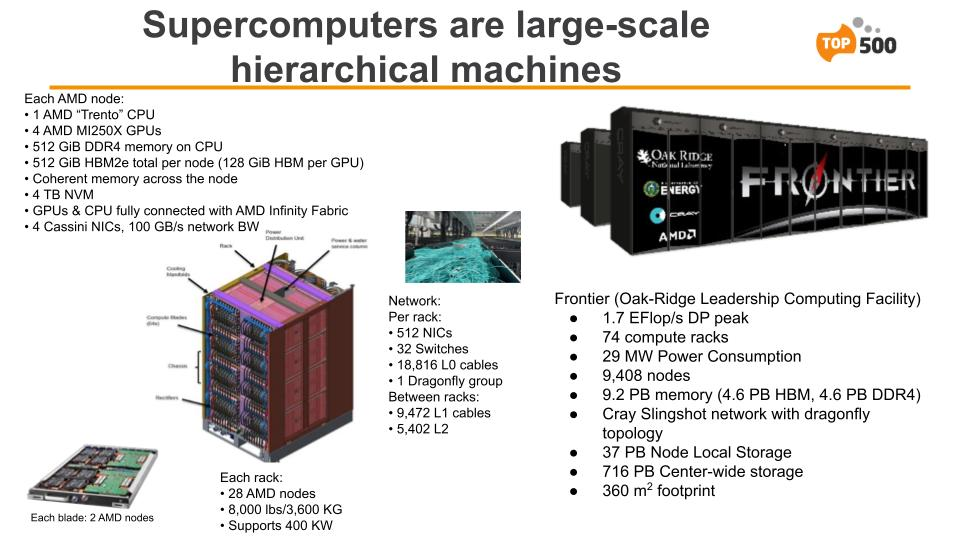
\includegraphics[width=\textwidth]{figures/frontier-architecture.jpg}

  \begin{overlayarea}{\linewidth}{0cm}
    \only<2>{%
      \vspace{-8cm}
      \begin{center}
        \begin{minipage}{.7\linewidth}
          \begin{block}{What are those system used for?}
            Scientific simulation and computing
            
            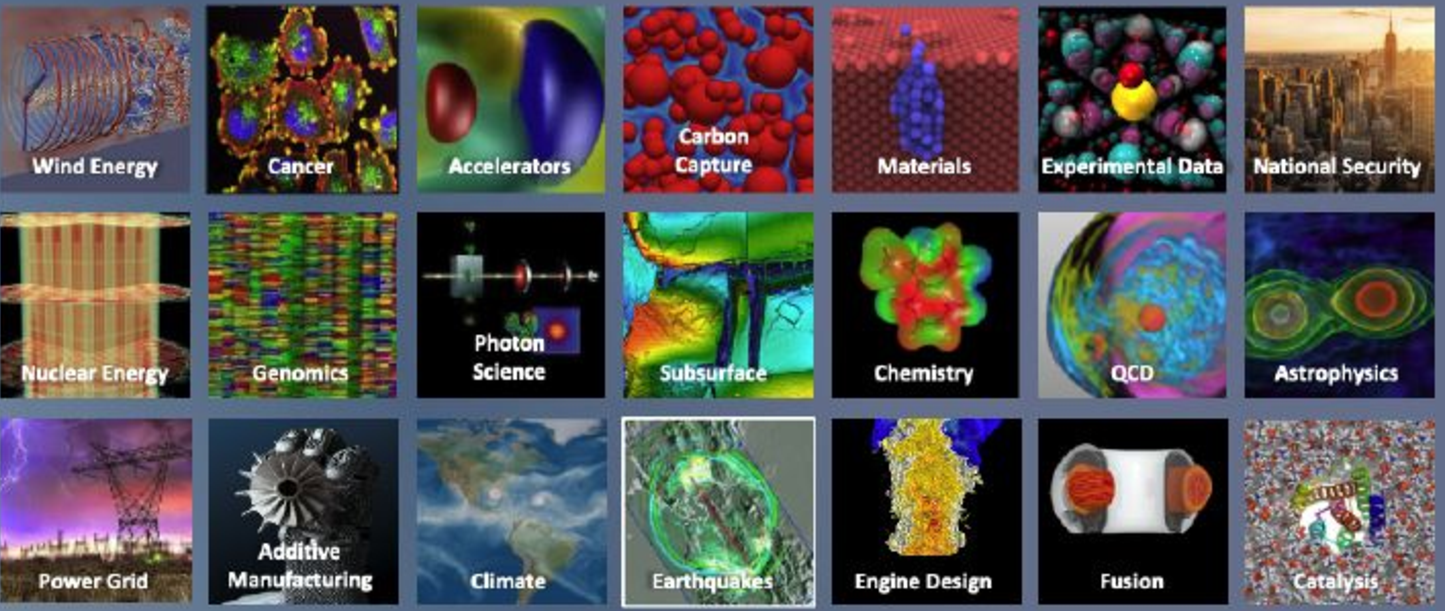
\includegraphics[width=\linewidth]{figures/hpc-applications.png}
          \end{block}
        \end{minipage}
      \end{center}
    }
  \end{overlayarea}
}

\frame{
  \includegraphics[width=\textwidth]{figures/top500.jpg}
}

\frame{
  \frametitle{Focus of this talk}

  Resilience techniques for High Performance Computing
  \begin{itemize}
  \item Rollback-recovery protocols
    \begin{itemize}
    \item Coordinated rollback-recovery
    \item Noncoordinated rollback-recovery
    \item Hierarchical protocols
    \end{itemize}
  \item Application-specific fault-tolerance
    \begin{itemize}
    \item User-Level Failure Mitigation
    \item Failure detection and notification for HPC
    \item Early Returning Agreement for ULFM
    \end{itemize}
  \end{itemize}
}

\frame{
  \frametitle{Effect of Scale}

  \begin{center}
    \only<1>{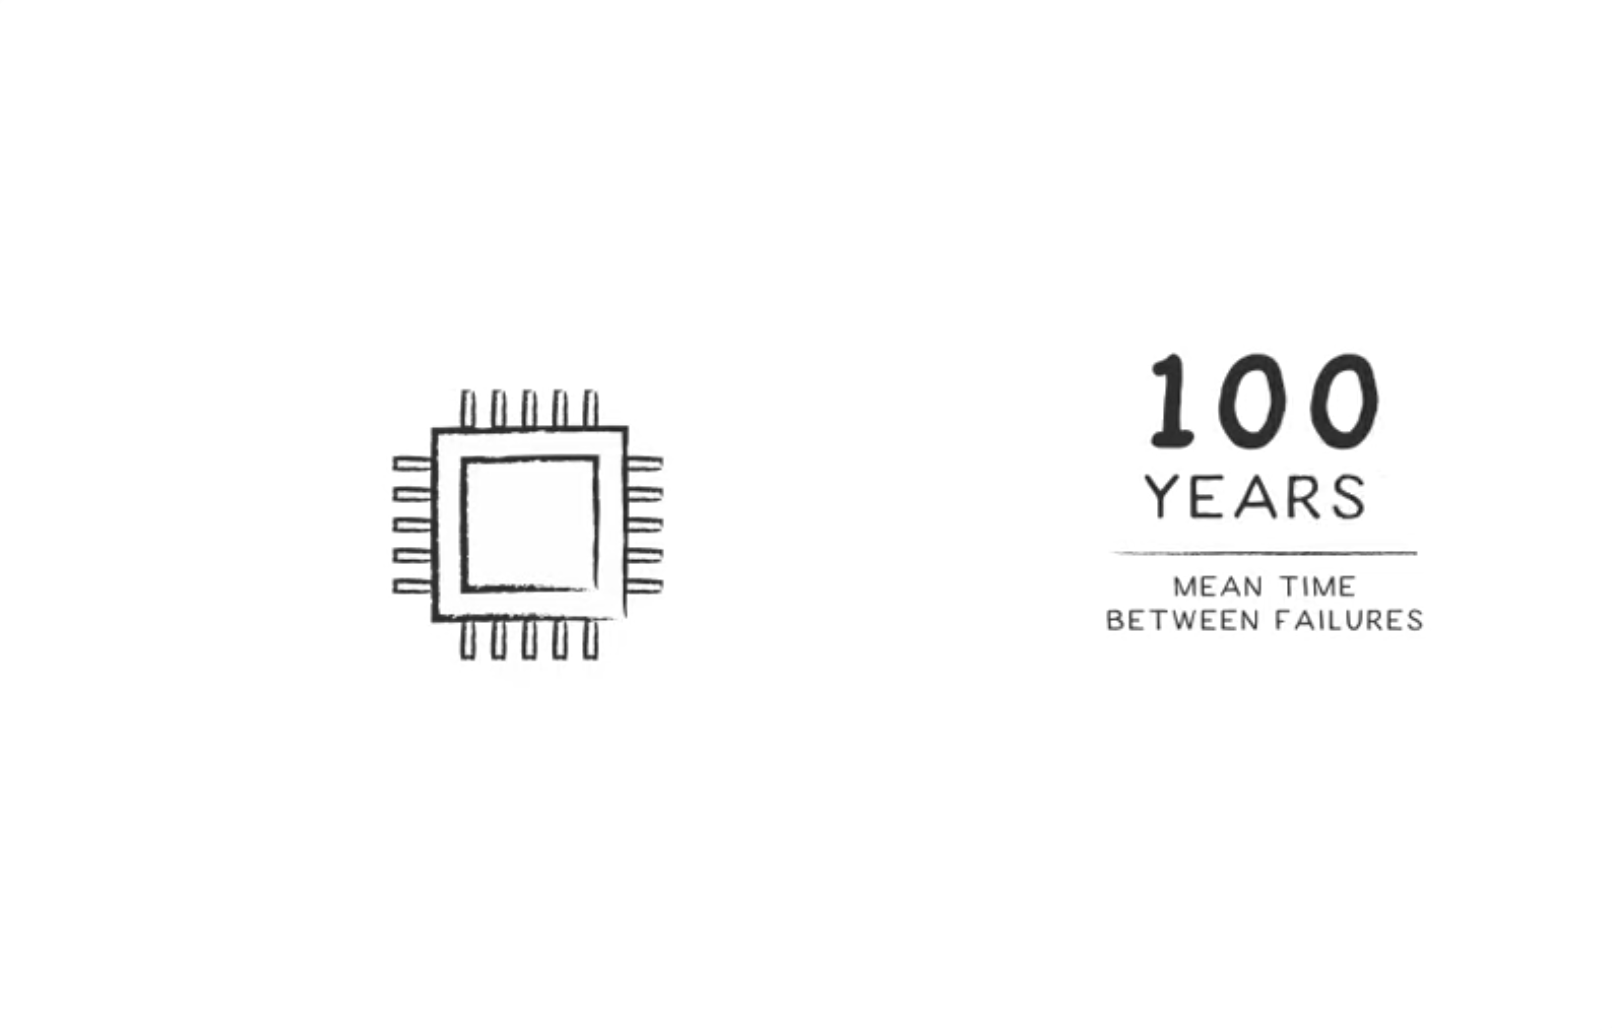
\includegraphics[width=.8\linewidth]{1_socket.png}}
    \only<2>{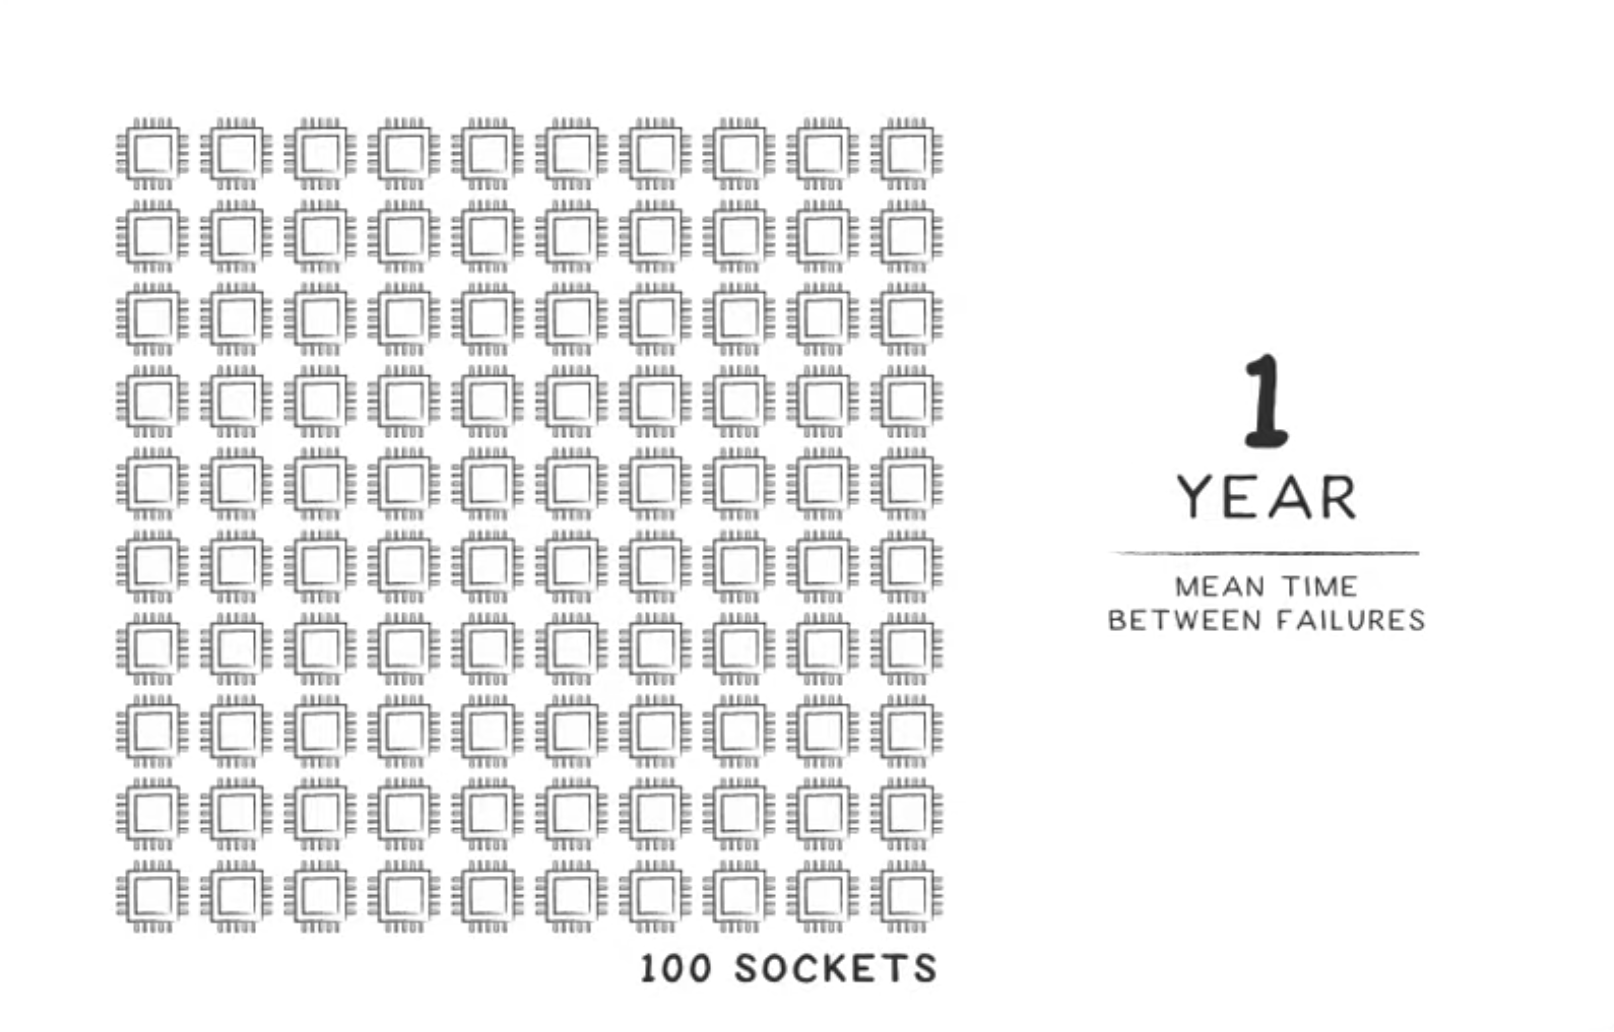
\includegraphics[width=.8\linewidth]{100_sockets.png}}
    \only<3>{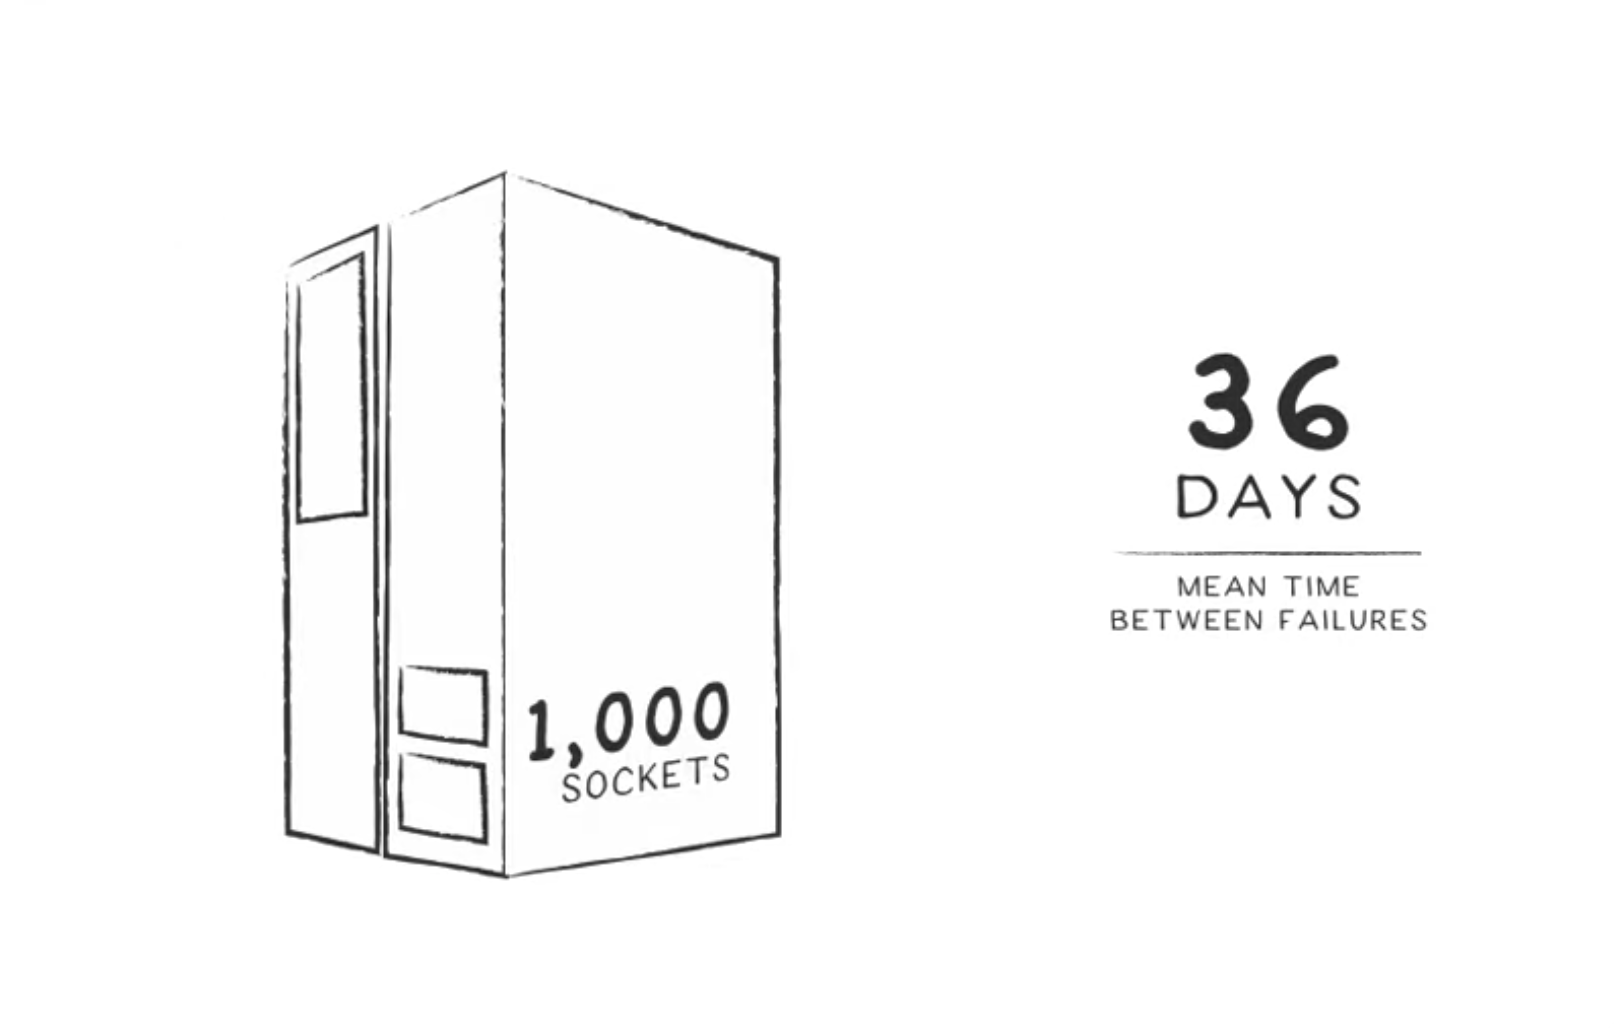
\includegraphics[width=.8\linewidth]{1000_sockets.png}}
    \only<4>{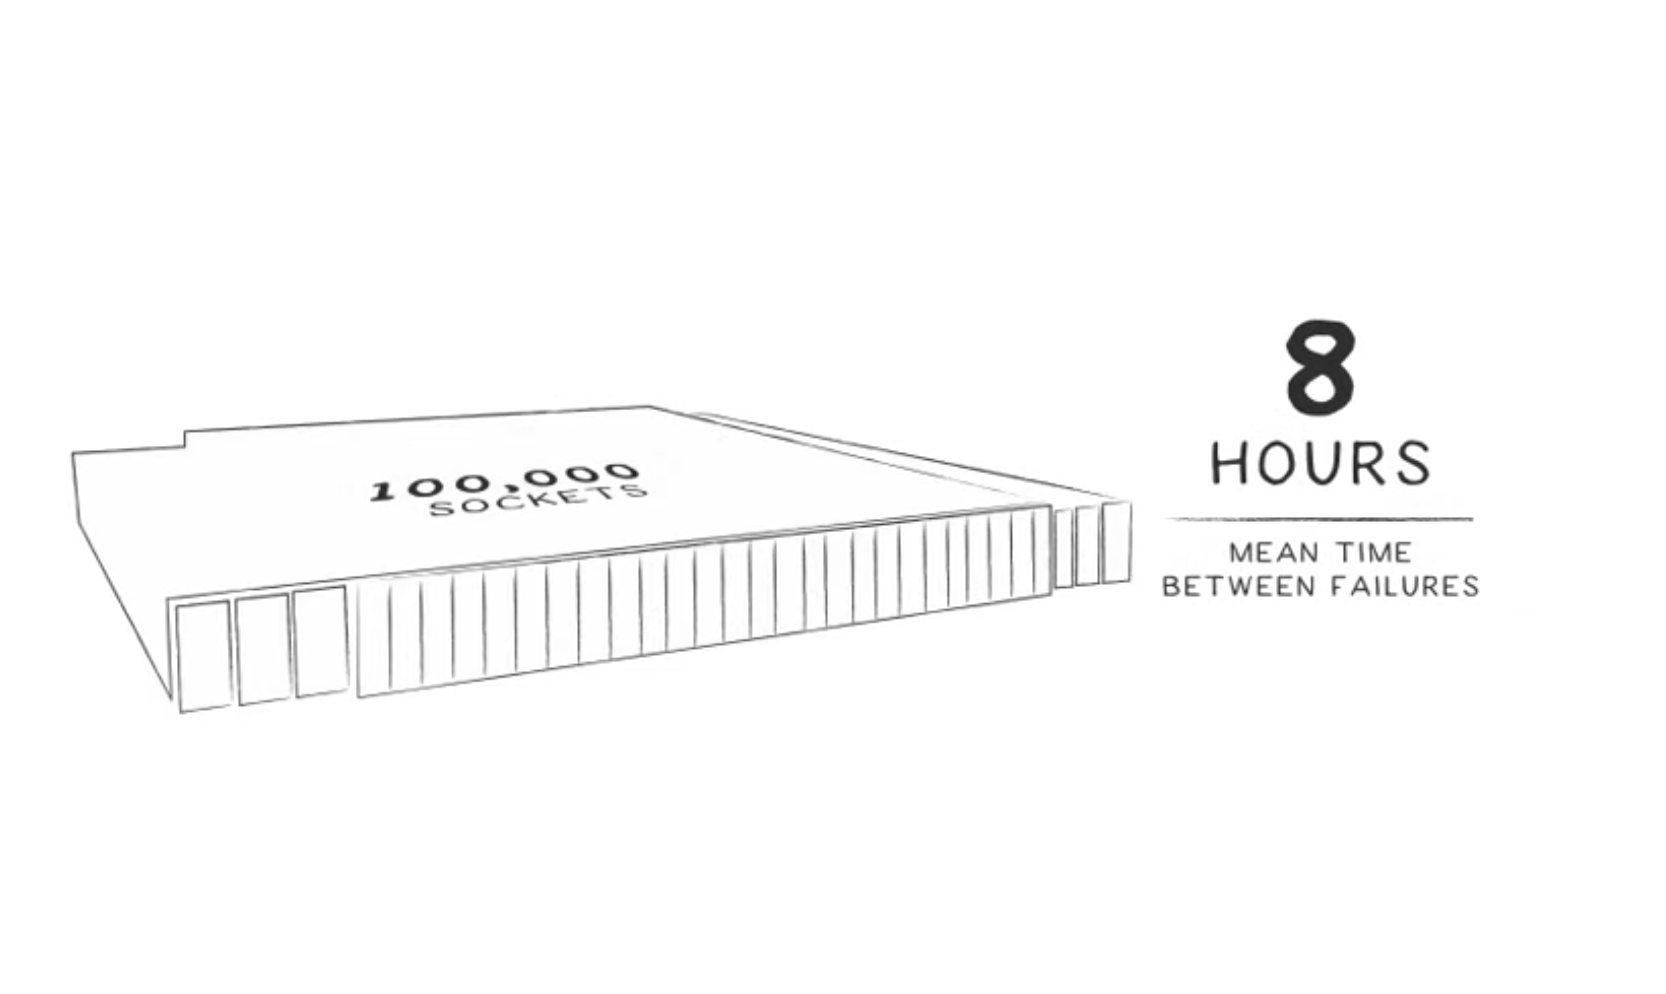
\includegraphics[width=.8\linewidth]{100000_sockets.png}}
  \end{center}
}

\frame{
  \frametitle{Petascale Computing Platforms}

  \begin{center}
    \includegraphics[width=.8\linewidth]{top500.jpg}
  \end{center}

    \begin{overlayarea}{\linewidth}{0cm}
    \only<2>{%
      \vspace{-6cm}
      \begin{center}
        \begin{minipage}{.7\linewidth}
          \begin{block}{Few Studies on the reliability of Petascale Systems}
            Not many traces and studies of Large-scale Computing Platforms
            reliability

            Not all studies look at simple characteristics (\emph{e.g.},
            MTBF):
            {\footnotesize\begin{itemize}
            \item Only \emph{Applications} failures
            \item Only \emph{Hardware} failures
            \item \emph{Logged events}
            \end{itemize}}
          \end{block}
        \end{minipage}
      \end{center}
    }
  \end{overlayarea}%
}

\frame{
  \frametitle{Petascale Platforms -- K-Computer}

  \begin{textblock*}{10cm}(0.5cm,1cm)
    \begin{block}{}
      \footnotesize \#20 Top500 (June'19, Rmax = 10.510 PFlop/s);
     06/11 --- 08/19\\
     864 cabinets; 88,128 nodes; 705,024 cores; 1.34PBytes; 12.6 MW; 
    \end{block}
    
    \vspace*{-1em}

    \begin{exampleblock}{}
     \footnotesize \emph{Fumiyoshi Shoji, Shuji Matsui, Mitsuo Okamoto, Fumichika Sueyasu,
      Toshiyuki Tsukamoto, Atsuya Uno and Keiji Yamamoto.} \textbf{ Long term
      failure analysis of 10 petascale supercomputer}.  Poster at ISC'15
    \end{exampleblock}
  \end{textblock*}

  \begin{textblock*}{4cm}(11.5cm,1.2cm) % {block width} (coords)
    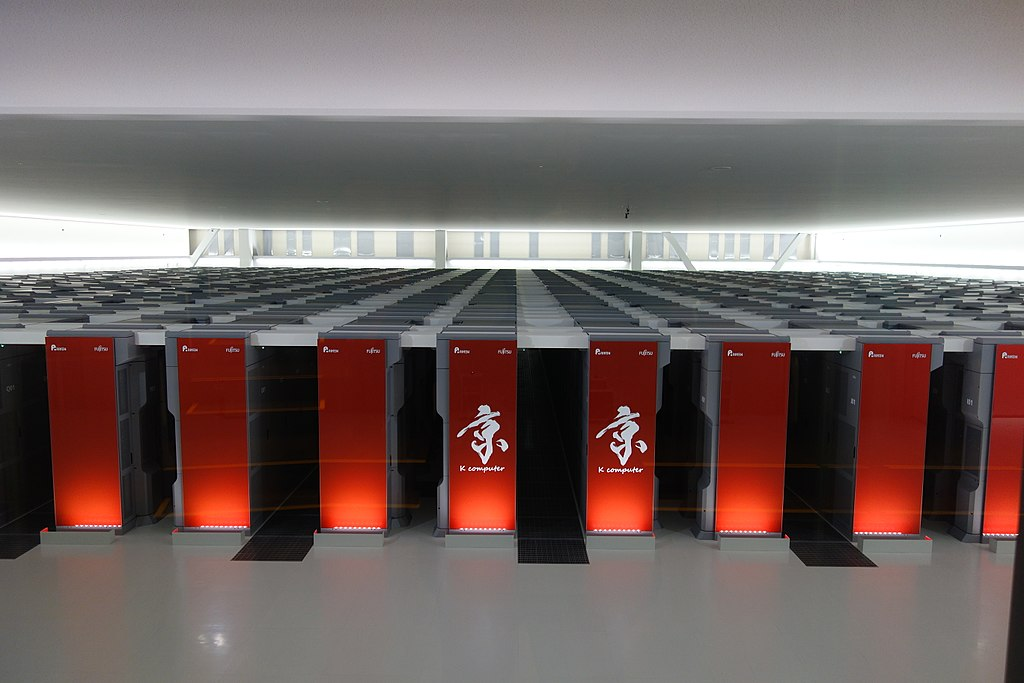
\includegraphics[width=4cm]{K-computer.jpg}
  \end{textblock*}

  \begin{textblock*}{.45\linewidth}(.02\linewidth,4.5cm)
    \small MFR = Monthly Failure Rate\\
    $\quad\qquad (= \frac{\textrm{\#failures during month}}{\textrm{\#unit total}})$

    \medskip

    \begin{tabular}{lccc}
      CPU MFR & $0.004\%$ &$\rightleftharpoons$ & $0.017\%$ \\
      DIMM MFR & $0.0017\%$ & $\searrow$ & $0.001\%$ \\
      Sys. Board MFR & $0.16\%$ & $\searrow$ & $0.05\%$\\
      \textcolor{red!40}{Sys. Board MTBF} & \textcolor{red!40}{1.1 day} & \textcolor{red!40}{$\nearrow$} & \textcolor{red!40}{3 day} \\
      \end{tabular}
  \end{textblock*}

  \begin{textblock*}{.45\linewidth}(.6\linewidth,4.5cm)
    \small AFR = Annualized Failure Rate\\
    $\quad\qquad (= 1-e^{\frac{-1 year}{MTBF}})$

    FIT = Failure In Time = \#fail. / $10^9$ h

    \bigskip

    \begin{tabular}{lcccc}
              & \# Parts & AFR & \textcolor{red!40}{MTBF} & FIT \\
      CPU & 82,944 & 0.06\% & \textcolor{red!40}{7.33 days} & 72.00 \\
      DIMM & 663,552 & 0.0016\% & \textcolor{red!40}{34.4 days} & 18.02 \\
      \end{tabular}
  \end{textblock*}

  \begin{textblock*}{.6\textwidth}(.58\textwidth,7.8cm)
    \scriptsize \textcolor{red!40}{(Numbers in red are derived from reported numbers in black)}
  \end{textblock*}
% K-computer: failure logs, CPU failures, DIMM failures, Storage
% Failures.
%   https://www.r-ccs.riken.jp/en/wp-content/uploads/sites/2/2015/11/Presentation.pdf
%  Monthly Failure Rate = Falilure count during month / number of installed (CPU|DIMM|SystemBoard)
%  CPUs Monthly failures: between 0.004% and 0.017%. Peaks at Gordon-Bell Challenges
%  DIMM Monthly failures: 0.0017% -> 0.0010% (air conditioner operations got improvement)
%  System Board MF: started at 0.16% decreased to 0.05%
%  Comparison with Blue Waters:
%    AFR = Annual Failure Rate -> K-computer 0.06%, Blue Waters 0.23%
%    FIT: Failure In Time (1 FIT = 1 failure per 10^9 hours of
%    computation on entire platform) -> K-computer 72, Blue Waters
%    265.15
%  For Blue waters see C. Di Martino et al., Lessons learned from the
%  analysis of system failures at petascale: the case of blue
%  waters. 44th international conference on Dependable Systems and
%  Networks (DSN 2014), 2014. 
%  System Availability: 93.59%, 4.19% scheduled maintenance, 2.23%
%  system failure.
%  Root cause: 1.38%/2.23% of file system.

}

\frame{
  \frametitle{Petascale Platforms -- Titan}

  \begin{textblock*}{10cm}(0.5cm,1cm)
    \begin{block}{}
      \footnotesize \#12 Top500 (June'19, Rmax = 17.590 PFlop/s);
     10/12 --- 08/19\\
     200 cabinets; 18,688 nodes; 299,008 cores; 18,688  K20X; 693.6TBytes; 8.2 MW; 
    \end{block}
  \end{textblock*}
    
  \begin{textblock*}{15cm}(0.5cm,2.5cm)
    \begin{exampleblock}{}
     \footnotesize \emph{R. A. Ashraf and C. Engelmann,} \textbf{Analyzing the
     Impact of System Reliability Events on Applications in the Titan
     Supercomputer}, 8th Workshop on Fault Tolerance for
     HPC at eXtreme Scale (FTXS), 2018
    \end{exampleblock}
  \end{textblock*}

  \begin{textblock*}{4cm}(11.5cm,1.2cm) % {block width} (coords)
    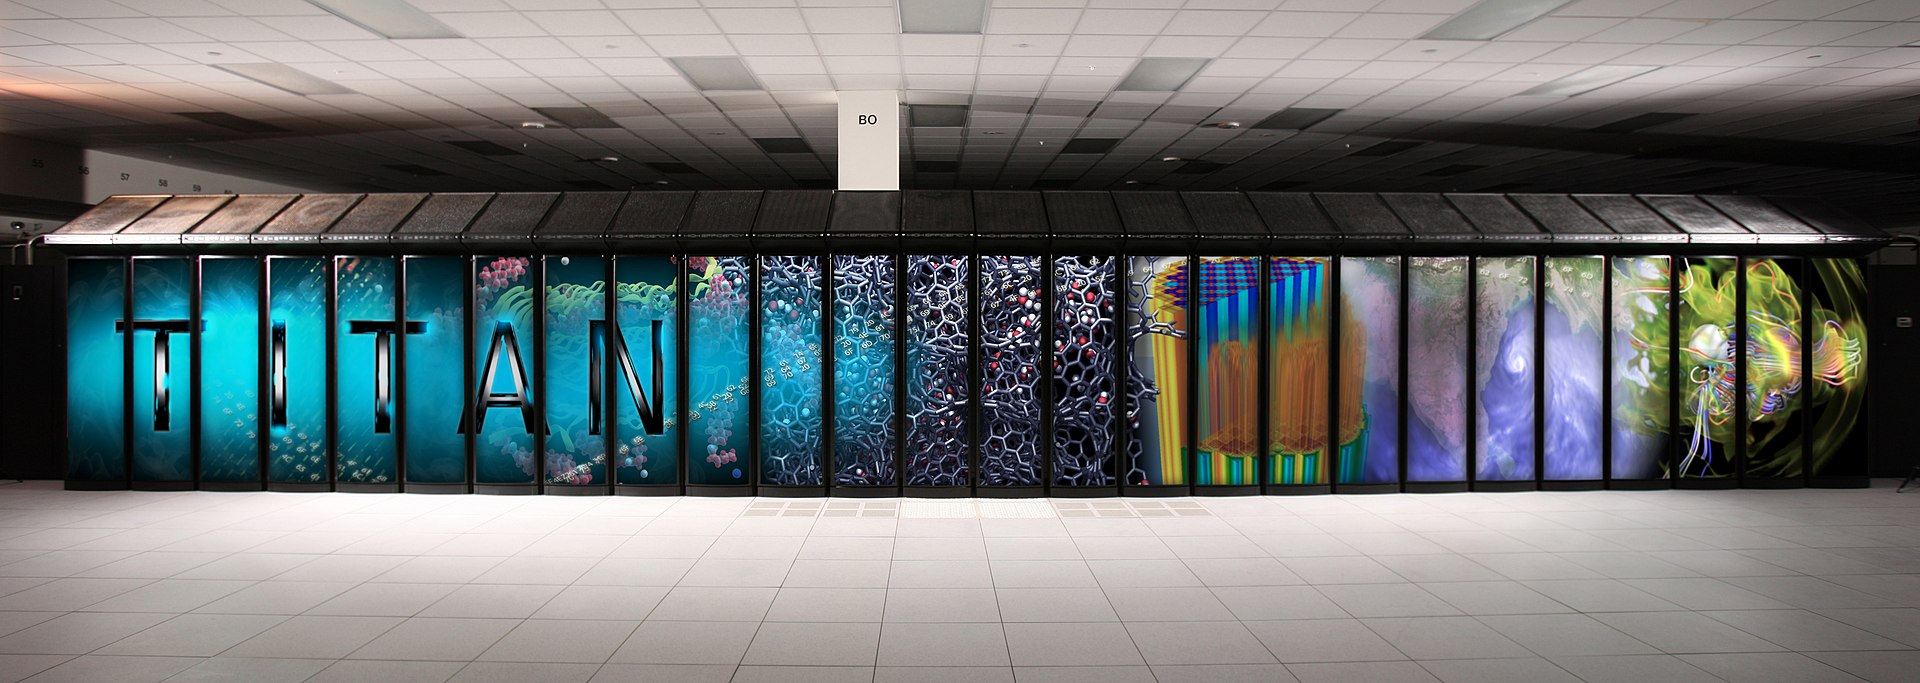
\includegraphics[width=4cm]{Titan.jpg}
  \end{textblock*}

  \begin{textblock*}{.5\linewidth}(.02\linewidth,4cm)
    Event log from Reliability, Availability and Serviceability (RAS)
    System

    \medskip
    $68k$ apps have $1+$ events (over $2\cdot 10^6$)

    \medskip\small
    95\% of apps with 11k+ nodes have $1+$ events

    91\% of apps with 125- nodes have 0 events

    85\% apps under 30min have 0 events

    80\% apps above 24h have $1+$ events
  \end{textblock*}

  \begin{textblock*}{.45\linewidth}(.6\linewidth,4cm)
    Nature of first event hitting an application:
    \begin{tabular}{ll}
      Parallel Filesystem & 73.7\%\\
      Processor Failure & 15.7 \%\\
      Machine Check Exception & 6.5\%\\
      GPU Failure & 1.5\%\\
      OOM / SEGFAULT & 1.9\%\\
      Interconnect & 0.8 \%
    \end{tabular}
  \end{textblock*}

% Titan Reliability
%   https://ieeexplore.ieee.org/abstract/document/8564486
% Evaluate events from RAS (Reliability, Availability and
% Serviceability) system. Eevents might not denote failure of 
% job. 68k applications / 2 million had an event reported.
% Events are also correlated: a FS failure often translates into a MCE
% failure and/or a Processor failure. GPU failure also, etc.
%   First event distribution:
%     Parallel FS: 73.7% of errors
%     Processor failures: 15.7%
%     Machine Check Exception (this includes masked failures, like
%     corrected ECC): 6.5%
%     GPU: 1.5%
%     OOM / SEGFAULT: 1.9%
%     Interconnect: 0.8%
%  95% of apps with 11250 to max nodes reported at least an event;
%  91% of apps in the 1 to 125 job size bin reported no event.
%  Similar story about duration: 85% of apps that are below 30min
%  reported no event 80% of apps above 24h reported an event
% 
}

\frame{
  \frametitle{Petascale Platforms -- Titan}

  \begin{textblock*}{10cm}(0.5cm,1cm)
    \begin{block}{}
      \footnotesize \#12 Top500 (June'19, Rmax = 17.590 PFlop/s);
     10/12 --- 08/19\\
     200 cabinets; 18,688 nodes; 299,008 cores; 18,688  K20X; 693.6TBytes; 8.2 MW; 
    \end{block}
  \end{textblock*}
    
  \begin{textblock*}{15cm}(0.5cm,2.5cm)
    \begin{exampleblock}{}
     \footnotesize \emph{E. Rojas, E. Meneses, T. Jones and D. Maxwell} \textbf{Analyzing a Five-year Failure Record of a
Leadership-class Supercomputer}, 31st Intl. Symp. on Computer Architecture and HPC (SBAC-PAD), 2019
    \end{exampleblock}
  \end{textblock*}

  \begin{textblock*}{4cm}(11.5cm,1.2cm) % {block width} (coords)
    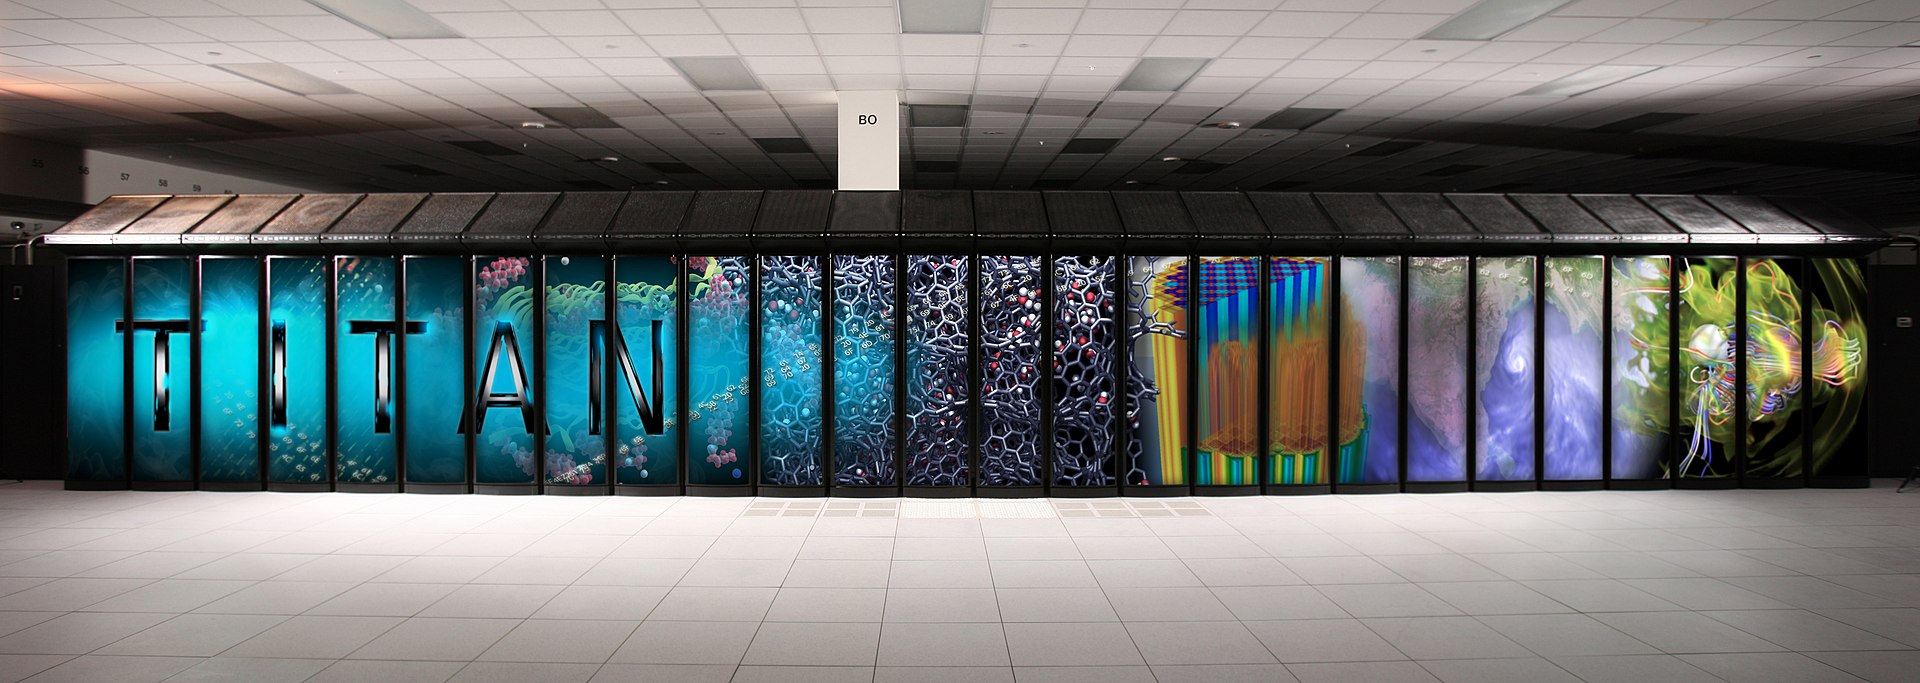
\includegraphics[width=4cm]{Titan.jpg}
  \end{textblock*}

  \begin{textblock*}{.5\linewidth}(.02\linewidth,4cm)
    System failure database (sys. admin.)

    {\small
    \begin{tabular}{c|ccccc}
      Year & 2014 & 2015 & 2016 & 2017 & 2018\\\hline
      Events & 161k & 258k & 444k & 452k & 1,348k \\\hline
    \end{tabular}}
    {\tiny (About 30\% of events are categorized as having a user origin)}

    \medskip
    %Several (potentially many) events may represent a single failure.
    5,625 hardware failures / 4 years ($\approx$4/day -- \textcolor{red!40}{6h MTBF})\\

    %\medskip
    %816,826 events (30.7\%) categorized as user, removed from the
    %analysis

    \medskip
    GPU DBE represents 53\% of hardware events
    {\small
    ECC on these GPUs
    is single error correction double error detection, leads to interrupt
    in DBE.}
 \end{textblock*}

  \begin{textblock*}{.45\linewidth}(.6\linewidth,4cm)
    Nature of failure:
    \begin{tabular}{ll}
      GPU DBE & 2070 (37\%)\\
      GPU BUS & 797 (14\%)\\
      GPU DPR & 308 (5.5\%)\\
      GPU XID (Soft.) & 1370 (24\%)\\
      Machine Check Exc & 653 (12\%)\\
      Other Failures & 427 (7.5\%)
    \end{tabular}
  \end{textblock*}

  \begin{textblock*}{.6\textwidth}(.58\textwidth,7.8cm)
    \scriptsize \textcolor{red!40}{(Numbers in red are derived from reported numbers in black)}
  \end{textblock*}

% Titan Reliability 2
%   https://ieeexplore.ieee.org/stamp/stamp.jsp?tp=&arnumber=8924181
% Evaluate events from a database of errors collected between 2014 and 2018.
% Correlate with jobs database and return code, and separate system errors
% from user errors.
%  68k applications / 2 million had an event reported.
% Events are also correlated: a FS failure often translates into a MCE
% failure and/or a Processor failure. GPU failure also, etc.
%   First event distribution:
%     Parallel FS: 73.7% of errors
%     Processor failures: 15.7%
%     Machine Check Exception (this includes masked failures, like
%     corrected ECC): 6.5%
%     GPU: 1.5%
%     OOM / SEGFAULT: 1.9%
%     Interconnect: 0.8%
%  95% of apps with 11250 to max nodes reported at least an event;
%  91% of apps in the 1 to 125 job size bin reported no event.
%  Similar story about duration: 85% of apps that are below 30min
%  reported no event 80% of apps above 24h reported an event
% 
}


\begin{frame}
  \frametitle{Petascale Platforms -- Sunway TaihuLight}

  \begin{textblock*}{10cm}(0.5cm,1cm)
    \begin{block}{}
      \footnotesize \#3 Top500 (June'19, Rmax = 93.014 PFlop/s);
     06/16 --- \\
     40 cabinets; 20,480 nodes; 10,649,600 cores; 1.32PBytes; 15 MW; 
    \end{block}
  \end{textblock*}
    
  \begin{textblock*}{10cm}(0.5cm,2cm)
    \begin{exampleblock}{}
     \footnotesize \emph{Liu RT, Chen ZN.} \textbf{A large-scale study of failures on
     petascale supercomputers.} Journal of Computer Science and
   Technology 33(1): 24-41, Jan. 2018
    \end{exampleblock}
  \end{textblock*}

  \begin{textblock*}{4cm}(11.5cm,1.2cm) % {block width} (coords)
    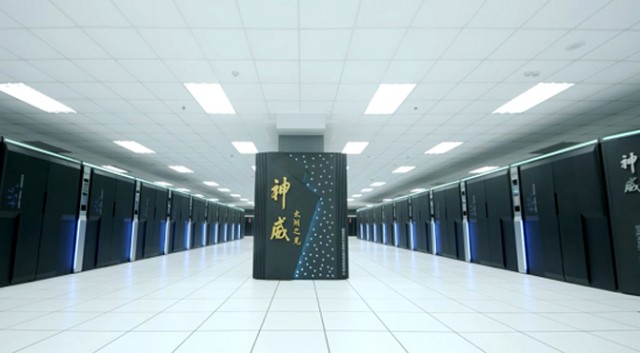
\includegraphics[width=4cm]{taihulight.jpg}
  \end{textblock*}

  \begin{textblock*}{.5\linewidth}(.02\linewidth,4cm)
    \footnotesize Nature of faults:
    \begin{tabular}{lll}
                & All Failures & Fatal Failures\\
      CPU       & 40\%         & 68\% \\
      Memory    & 48\%         & 21\% \\
      Power     & 9\%          & 5\%\\
      MD$^{(*)}$ & 2\%          & 5\% \\
    \end{tabular}

    {\scriptsize ($(*)$ MD: Maintenance and Diagnosis system)}

    \medskip
    Effect of Application (1 cabinet, \#faults/month):
    \begin{tabular}{lll}
                     & Mem Faults                   & CPU Faults \\
        Comp. only   & $7 \rightleftharpoons 93$    & $5 \rightleftharpoons 33$ \\
        Comp. \& Mem & $527 \rightleftharpoons 995$ & $136 \rightleftharpoons 867$ \\
        Comm. \& Mem & $115 \rightleftharpoons 284$ & $20 \rightleftharpoons 85$
    \end{tabular}
  \end{textblock*}

  \begin{textblock*}{.45\linewidth}(.6\linewidth,4cm)
    {\small 3 time spans; 1 CPU; 2 Computing Cards}
    Weibull Distribution best fits CDF

    \medskip
    \begin{tabular}{llll}
                    & $P_1$    & $P_2$  & $P_3$ \\
      $CPU_1$ MTBF  & 8 days   & 4 days & 10 days\\
      $Card_1$ MTBF & 9.5 days &        & \\
      $Card_2$ MTBF & 10 days  &        & \\
    \end{tabular}

    \medskip
    {\scriptsize\textcolor{red!40}{Data too sparse to give a system MTBF}}\\
    {\scriptsize\textcolor{red!40}{It was probably small}}
        
    {\tiny MTBF computed from $\eta$ and $m$ parameters
      given in the article:\\
      PDF: $f(x) = \frac{m}{\eta}(\frac{x}{\eta})^{m-1}e^{-(x/\eta)^m}$;\\
      MTBF: $=\eta\, \Gamma(1+1/m)$}
    
  \end{textblock*}

% A large scale study of failures on petascale supercomputers (2018):
% https://link.springer.com/content/pdf/10.1007%2Fs11390-018-1806-7.pdf
%  Sunway BlueLight (based on multi-core CPUs) and Sunway TaihuLigh
%  (based on heterogeneous manycore CPUs
% They conclude that a Weibull distribution always fits best both machines,
% but the parameters depends strongly on the workload. For example, on 
% CPU failures, for Sunway TaihuLigh they take 3 random intervals
% (epochs) and find:
%   -> MTBF = eta * Gamma(1 + 1/m) = 690434s (8 days) during 'epoch 1'
%            351001s (4 days) during 'epoch 2'
%            906820s (10 days) during 'epoch 3'
% Looking at the interconnect level, they find a Time Between Failure
%  between 824082.3s (9.5 days) and 9.08.10^5s (10 days).
%  Sunway BlueLigh: 91.99 of all notifications are memory events,
%    44.48% of fatal errors are due to CPU
%    41.67% of fatal errors are due to Interconnect
%    9.36% of fatal errors are due to power supply
%   Only 1.03% fatal errors are due to memory.
% Sunway TaihuLigh: 48% of nonfatal & Fatal are due to Memory, 40% are
% due to CPU, and 9% to Power
%     Fatal errors: 68% due to CPU, 21% to memory 5% to power
%
\end{frame}

%% \begin{frame}
%%   \frametitle{In the recent past}
  
%%   \begin{center}
%%     \relsize{-1}
%%     \begin{tabular}{l|l|l|l|l|l}
%%       System & \#Nodes & \#cores & Period & MTBF (h) & Scale-Norm. MTBF (h) \\\hline
%%       Jaguar XT4 & 7,832  & 31,328  & Jan'08-Mar'11 & 36.91 & 15.47 \\\hline
%%       Jaguar XT5 & 18,688 & 149,504 & Jan'09-Dec'11 & 22.67 & 22.67 \\\hline
%%       Jaguar XK6 & 18,688 & 298,592 & Jan'12-Oct'12 & 8.93  &  8.93 \\\hline
%%       Eos XC 30 & 736     & 23,553  & Sep'13-Sep'15 & 189.04 & 7.45 \\\hline
%%       Titan XK7 & 18,688  & 560,640 & May'13-Sep'15 & 14.51  & 14.51 \\
%%     \end{tabular}

%%     \medskip

%%     \relsize{-1} Table 2 + 3 of ``Failures in Large Scale Systems: Long-term Measurement, Analysis, and Implications'',\\
%%     by S. Gupta, T. Patel, C. Engelmann, and D. Tiwari, SC'17
%%   \end{center}

%%   \bigskip

%%   \noindent$\bullet$ Reliability does not seem to be correlated with size or 'age' of the machine\\
%%   $\bullet$ A few failure types constitute a major fraction of all failures.\\
%%   $\bullet$ Temporal recurrences are observed
  
%% \end{frame}

\frame{
  \frametitle{Exascale platforms (courtesy Jack Dongarra)}

  \centerline{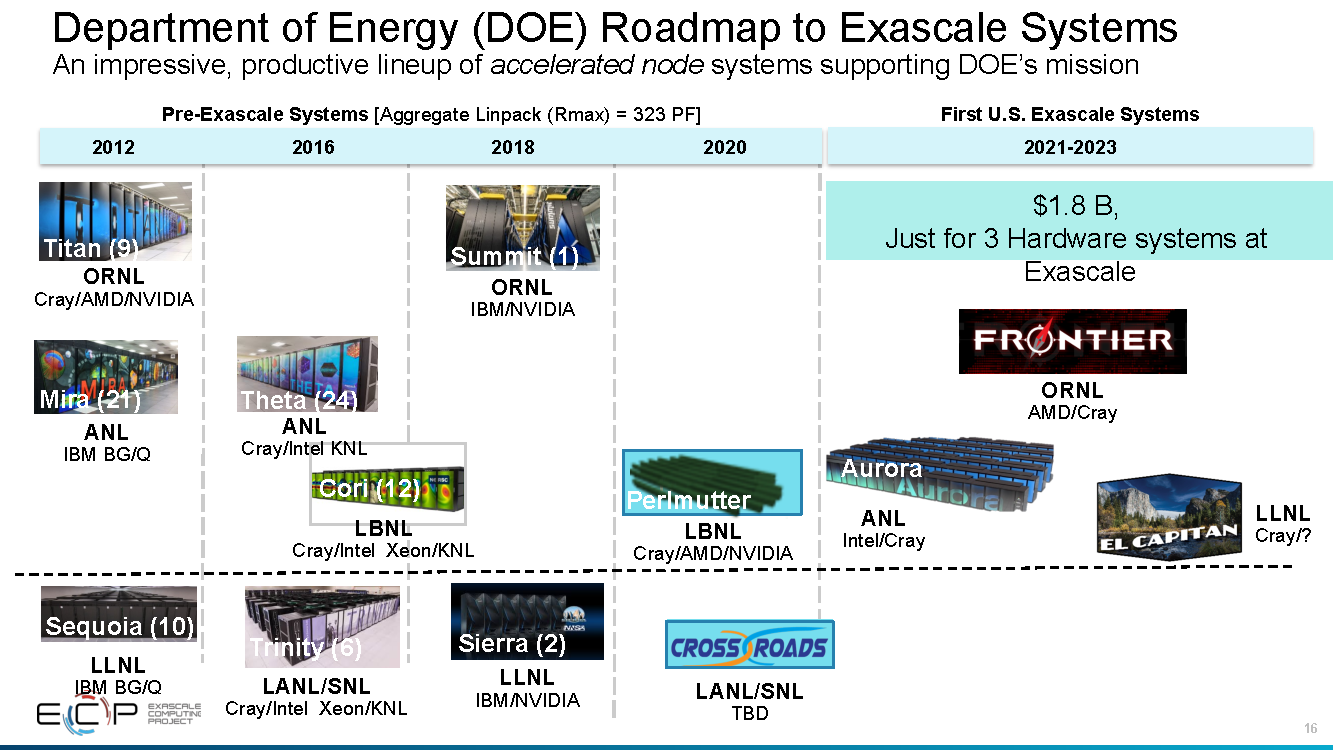
\includegraphics[width=1.4\textheight]{DOE-Exascale-Roadmap.pdf}}

  \begin{overlayarea}{\linewidth}{0cm}
    \only<2>{%
      \vspace{-6cm}
      \begin{center}
        \begin{minipage}{.7\linewidth}
          \begin{block}{Fewer Studies on the reliability of Pre-Exascale Systems}

            \begin{itemize}
            \item MTBF of \textcolor{blue}{systems} appear to remained capped
            \item \# nodes in Top10 has \emph{decreased}
            \item Computing power of nodes has significantly increased thanks to \emph{many GPUs} / node
              \begin{itemize}
              \item Notable exceptions:
              \item[] $\qquad$ K-Computer, Fugaku
              \item[] $\qquad$ Sunway *light
              \end{itemize}
            \end{itemize}
          \end{block}
        \end{minipage}
      \end{center}
    }
  \end{overlayarea}%

}

